\documentclass[a4paper]{article}

%Tutti gli usepackage vanno qui

\usepackage{geometry}
\usepackage[italian]{babel}
\usepackage[utf8]{inputenc}
\usepackage[T1]{fontenc}
\usepackage{tgschola}
%\usepackage{tgbonum}
\usepackage{tabularx}
\usepackage{longtable}
\usepackage{hyperref}
\usepackage{enumitem}
\usepackage[toc]{appendix}
\hypersetup{
	colorlinks=true,
	linkcolor=black,
	filecolor=magenta,      
	urlcolor=blue,
}
% Numerazione figure 
\let\counterwithout\relax
\let\counterwithin\relax
\usepackage{chngcntr}

\counterwithin{table}{subsection}
\counterwithin{figure}{subsection}

\usepackage[bottom]{footmisc}
\usepackage{fancyhdr}
\setcounter{secnumdepth}{4}
\usepackage{amsmath, amssymb}
\usepackage{array}
\usepackage{graphicx}

\usepackage{ifthen}

%\usepackage{float}
\usepackage{layouts}
\usepackage{url}
\usepackage{comment}
\usepackage{float}
\usepackage{eurosym}

\usepackage{lastpage}
\usepackage{layouts}
\usepackage{float}
\usepackage{eurosym}

%Comandi di impaginazione uguale per tutti i documenti
\pagestyle{fancy}
\lhead{
\includegraphics[scale=0.04]{../../../../latex/images/logoTWM.png}}
%Titolo del documento
\rhead{\doctitle{}}
%\rfoot{\thepage}
\cfoot{Pagina \thepage\ di \pageref{LastPage}}
\setlength{\headheight}{35pt}
\setcounter{tocdepth}{5}
\setcounter{secnumdepth}{5}
\renewcommand{\footrulewidth}{0.4pt}

% multirow per tabelle
\usepackage{multirow}

% Permette tabelle su più pagine
%\usepackage{longtable}


% colore di sfondo per le celle
\usepackage[table]{xcolor}

%COMANDI TABELLE
\newcommand{\rowcolorhead}{\rowcolor[HTML]{9b240a}} %intestazione 
% check for missing commands
\newcommand{\headertitle}[1]{\textbf{\color{white}#1}} %titolo colonna
\definecolor{pari}{HTML}{FFDBCB}
\definecolor{dispari}{HTML}{F1F7FD}

% comandi glossario
\newcommand{\glo}{$_{G}$}
\newcommand{\glosp}{$_{G}$ }


%label custom
\makeatletter
\newcommand{\uclabel}[2]{%
	\protected@write \@auxout {}{\string \newlabel {#1}{{#2}{\thepage}{#2}{#1}{}} }%
	\hypertarget{#1}{#2}
}
\makeatother

%riportare pezzi di codice
\definecolor{codegray}{gray}{0.9}
\newcommand{\code}[1]{\colorbox{codegray}{\texttt{#1}}}



% Configurazione della pagina iniziale
\newcommand{\doctitle}{Norme di Progetto}
\newcommand{\docdate}{ } % lasciare vuoto (uno carattere di spazio) per i documenti che non sono verbali, così non viene scritta la data
\newcommand{\rev}{3.0.1}
\newcommand{\stato}{Non Approvato}
\newcommand{\uso}{Interno}
\newcommand{\approv}{--De Renzis Simone}
\newcommand{\red}{Greggio Nicolò\\& Tessari Andrea}
\newcommand{\ver}{Zuccolo Giada\\& Crivellari Alberto}
\newcommand{\dest}{Three Way Milkshake\\ Prof. Vardanega Tullio\\ Prof.
 Cardin Riccardo}
\newcommand{\describedoc}{Questo documento contiene tutte le norme di progetto\textsubscript{G}, definite inizialmente o aggiunte in seguito, viene quindi aggiornato per incrementi successivi.}



 % modifica questo file
\makeindex

\usepackage{hyperref}
\hypersetup{
    colorlinks=true,
    linkcolor=blue,
    urlcolor=blue,
    hyperfootnotes=false
}
\usepackage{verbatim}
\usepackage{multicol}

\usepackage[toc,acronym]{glossaries}
\makeglossaries

\newglossaryentry{wiki}{name={wiki}, plural={wikis},%
	description={Termine di origine hawaiana che significa veloce, con cui si identifica un tipo di sito internet che permette la creazione e la modifica di pagine multimediali attraverso un'interfaccia semplice}}

\newglossaryentry{vmodel}{name={Modello a V},%
	description={Modello che illustra le relazioni tra ogni fase del ciclo di vita del software con la relativa fase di testing ad essa associata}}

\newglossaryentry{usecase}{name={caso d'uso}, plural={casi d'uso},%
	description={Un caso d'uso è un insieme di \glspl{scenario} che hanno in comune uno scopo finale (obiettivo) per un utente (\gls{attore})}}

\newglossaryentry{techbase}{name={technology baseline},%
	description={Motiva le tecnologie, i framework, e le librerie selezionate per la realizzazione del prodotto. Ne dimostra adeguatezza e fattibilità, tramite un proof of concept coerente con gli obiettivi}}

\newglossaryentry{task}{name={task}, plural={tasks},%
	description={Nel contesto del capitolato, con questo termine si identifica un compito da svolgere da parte di un unità (muletto) che consiste nel raggiungere un \acrshort{POI} e caricare o scaricare la merce}}

\newglossaryentry{stakeholder}{name={stakeholder}, plural={stakeholders},%
	description={Tutti coloro che a vario titolo hanno influenza sul prodotto e sul progetto. Sono stakeholders il committente, il proponente, gli utenti, il team di sviluppo}}

\newglossaryentry{sistematico}{name={sistematico},%
	description={Modo di lavorare metodico e rigoroso, che conosce, usa ed evolve le best practice di dominio}}

\newglossaryentry{shell}{name={shell},%
	description={Interprete dei comandi}}

\newglossaryentry{security}{name={security},%
	description={Non vulnerabilità rispetto a intrusioni}}

\newglossaryentry{scenario}{name={scenario}, plural={scenari},%
	description={Nell'ambito dello sviluppo software, sequenza di passi che descrive l'interazione tra l'\gls{attore} e il sistema, e le elaborazioni necessarie per soddisfare la richiesta dell'\gls{attore}}}

\newglossaryentry{safety}{name={safety},%
	description={Sicurezza rispetto a malfunzionamenti}}

\newglossaryentry{risorsa}{name={risorsa}, plural={risorse},%
	description={Mezzo o capacità disponibile, nello sviluppo software ad esempio le persone, il tempo, il denaro, gli strumenti necessari allo sviluppo del progetto. Le attività di progetto consumano le risorse disponibili}}

\newglossaryentry{revisione}{name={revisione}, plural={revisioni},%
	description={Esame o controllo, per lo più periodico, inteso a verificare il grado dell'efficienza, della funzionalità, della corrispondenza a determinati requisiti. Nell'ambito del corso di Ingegneria del Software, la revisione di avanzamento identifica il momento in cui il team consegna e presenta gli artefatti sviluppati durante il periodo appena trascorso}}

\newglossaryentry{requisito}{name={requisito}, plural={requisiti},%
	description={Esistono due interpretazioni principali di un requisito \begin{itemize}\item dal lato del bisogno(ovvero il cliente/utente) è la capacità necessaria a un utente per risolvere un problema o raggiungere un obiettivo\item dal lato della soluzione (ovvero lo sviluppatore) è la capacità che deve essere posseduta (o condizione che deve essere soddisfatta) da un sistema per adempiere a un obbligo \end{itemize}}}

\newglossaryentry{repository}{name={repository},%
	description={Posizione di archiviazione per pacchetti software}}

\newglossaryentry{quantificabile}{name={quantificabile},%
	description={Che permette di misurare l'efficienza e l'efficacia del suo agire}}

\newglossaryentry{proofconcept}{name={proof of concept},%
	description={Dimostratore eseguibile. Il suo codice può (ma non deve) essere usa-e-getta}}

\newglossaryentry{progetto}{name={progetto}, plural={progetti},%
	description={Insieme di attività che devono raggiungere determinati obiettivi a partire da determinate specifiche; hanno una data d'inizio e una data di fine fissate, dispongono di risorse limitate e consumano tali risorse nel loro svolgersi}}

\newglossaryentry{prodbase}{name={product baseline},%
	description={Illustra la baseline architetturale del prodotto, coerente con la \acrshort{tb}. Rappresenta il design definitivo}}

\newglossaryentry{precondizione}{name={precondizione}, plural={precondizioni},%
	description={Condizioni che devono essere soddisfatte affinché si verifichino determinati eventi successivi}}

\newglossaryentry{postcondizione}{name={postcondizione}, plural={postcondizioni},%
	description={Condizioni che devono verificarsi dopo determinati eventi}}

\newglossaryentry{planimetria}{name={planimetria}, plural={planimetrie},%
	description={Rappresentazione in piano del magazzino che ne evidenzia le caratteristiche (aree non transitabili, zone di percorrenza, punti di interesse)}}

\newglossaryentry{periodo}{name={periodo}, plural={periodi},%
	description={Nel contesto del documento, l'intervallo di tempo che intercorre tra due revisioni successive}}

\newglossaryentry{percorrenza}{name={percorrenza}, plural={percorrenze},%
	description={Nel contesto del capitolato, i vincoli relativi alle zone transitabili: \begin{itemize} \item sensi di marcia \item numero massimo di unità che vi possono transitare \end{itemize}}}

\newglossaryentry{modellosviluppo}{name={modello di sviluppo},%
	description={Principio teorico che indica il metodo da seguire nel progettare e nello scrivere un programma. Esistono tre principali modelli di sviluppo, ossia sequenziale, \gls{incrementale} ed evolutivo.}}

\newglossaryentry{milestone}{name={milestone},%
	description={Pietra miliare, istante temporale su cui si misura l'avanzamento del progetto. Viene fissata nel futuro per stabilire un avanzamento atteso. Una buona milestone è delimitata per ampiezza ed ambizioni, misurabile in termini di tempo e impegno necessario per raggiungerla, traducibile in compiti assegnabili ai membri del team e coerente con le scadenze del progetto}}

\newglossaryentry{kanban}{name={kanban},%
	description={Framework usato per implementare modelli di sviluppo Agili e DevOps. Richiede comunicazione in tempo reale tra i componenti de team e totale trasparenza. I work item vengono visualizzati su una Kanban Board, permettendo ai membri del team di vedere lo stato di ogni attività in ogni momento. Per maggiori dettagli \url{https://www.atlassian.com/agile/kanban/kanban-vs-scrum}}}

\newglossaryentry{incrementale}{name={incrementale},%
	description={Che procede per incrementi, ossia migliorie che, partendo da un impianto base, portano al raggiungimento dell'obiettivo producendo valore e limitando al massimo la regressione a stati già attraversati}}

\newglossaryentry{gitpush}{name={git-push},%
	description={Azione di git che permette di caricare le proprie modifiche locali sul server remoto condiviso del repository}}

\newglossaryentry{gitpull}{name={pull},%
	description={Comando di \gls{git} che permette di aggiornare il proprio \acrshort{repo} locale con i cambiamenti remoti}}

\newglossaryentry{git}{name={git},%
	description={Sistema di controllo del versionamento distribuito}}

\newglossaryentry{gitcommit}{name={commit}, plural={commits},%
	description={Comando di \gls{git} che permette di salvare e versionare le modifiche attuate ai file in locale}}

\newglossaryentry{gantt}{name={Gantt},%
	description={Diagramma per la pianificazione di un progetto. Esplicita le attività volte al suo svolgimento e per ognuna ne identifica data di inizio e di fine a seconda delle stime effettuate. Facilità la visualizzazione delle connessioni tra le attività e lo stato di avanzamento del progetto}}

\newglossaryentry{form}{name={form},%
	description={Interfaccia di un programma che consente a un utente di inserire e inviare uno o più dati}}

\newglossaryentry{fase}{name={fase}, plural={fasi},%
	description={Segmento temporale contiguo che che presuppone uno stazionamento in uno stato o in una transizione di ciclo di vita}}

\newglossaryentry{efficienza}{name={efficienza},%
	description={Misura dell'abilità di raggiungere l'obiettivo impiegando le risorse in maniera ottimale}}

\newglossaryentry{efficacia}{name={efficacia},%
	description={Misura della capacità di raggiungere l'obiettivo prefissato}}

\newglossaryentry{disciplinato}{name={disciplinato},%
	description={Che segue le regole che si è dato}}

\newglossaryentry{designpattern}{name={design pattern}, plural={design patterns},%
	description={Soluzione progettuale generale ad un problema ricorrente}}

\newglossaryentry{cruscotto}{name={cruscotto}, plural={cruscotti},%
	description={Interfaccia utente grafica che fornisce viste indicatori chiave di prestazione rilevanti per un particolare obiettivo o processo aziendale}}

\newglossaryentry{combobox}{name={combobox},%
	description={Controllo grafico (widget) che permette all'utente di effettuare una scelta scrivendola in una casella di testo o selezionandola da un elenco}}

\newglossaryentry{capitolato}{name={capitolato}, plural={capitolati},%
	description={Documento tecnico redatto dal cliente in cui vengono specificati i vincoli contrattuali (prezzo e scadenze) per lo sviluppo di un determinato prodotto software. Viene presentato in un bando d'appalto per trovare qualcuno che possa svolgere il lavoro richiesto}}

\newglossaryentry{bug}{name={bug},%
	description={Problema che porta al malfunzionamento del software, per esempio producendo un risultato inatteso o errato, tipicamente dovuto a un errore nella scrittura del codice sorgente di un programma}}

\newglossaryentry{bestpractice}{name={best practice}, plural={best practices},%
	description={Modo di fare noto, che abbia mostrato di garantire i migliori risultati in circostanze note e specifiche}}

\newglossaryentry{bash}{name={bash},%
	description={G:bash:bash:X:\gls{shell} Unix ed un linguaggio interpretato scritto da Brian Fox per il progetto GNU come sostituto del software gratuito per la shell Bourne}}

\newglossaryentry{baseline}{name={baseline},%
	description={Istantanea dello stato di avanzamento del progetto. Misura i risultati ottenuti e li fissa in una versione consolidata del prodotto. Può essere associata ad un rifermento temporale (\gls{milestone})}}

\newglossaryentry{attore}{name={attore}, plural={attori},%
	description={Ruolo interpretato da un utente (persona o sistema esterno) nei confronti del sistema. \begin{itemize} \item \textbf{attore primario}: attore richiede l'assistenza del sistema \item \textbf{attore secondario}: attore di cui è il sistema stesso a richiedere l'intervento \end{itemize}}}

\newglossaryentry{attivita}{name={attività},%
	description={Insieme di una o più azioni il cui completamento porta ad un avanzamento nel complesso}}

\newglossaryentry{artefatto}{name={artefatto}, plural={artefatti},%
	description={Sottoprodotto che viene realizzato durante lo sviluppo software. Sono artefatti i casi d'uso, i diagrammi delle classi, i modelli UML, il codice sorgente e la documentazione varia, che aiutano a descrivere la funzione, l'architettura e la progettazione del software}}

\newglossaryentry{agile}{name={agile},%
	description={Approccio stutturato e iterativo alla gestione dei progetti e alla sviluppo di software. Riconosce la volatilità dello sviluppo del prodotto e propone un metodo per permettere ai team di rispondere in maniera rapida a cambiamenti non pianificati e di produrre valore fin dalle prime iterazioni. Per maggiori dettagli \url{https://www.atlassian.com/agile/kanban/kanban-vs-scrum}}}

\newacronym{vcs}{VCS}{Version Control System}

\newacronym{uml}{UML}{Unified Modeling Language}

\newacronym{tb}{TB}{\gls{techbase}}

\newacronym{spa}{spa}{X}

\newacronym{rest}{REST}{REpresentational State Transfer}

\newacronym{repo}{repo}{\gls{repository}}

\newacronym{ram}{RAM}{Random Access Memory}

\newacronym{portacs}{PORTACS}{\acrshort{POI} Oriented Real Time Anti Collision System}

\newacronym{POI}{POI}{Point Of Interest}

\newacronym{poc}{PoC}{Proof of Concept}

\newacronym{pb}{PB}{\gls{prodbase}}

\newacronym{jit}{JiT}{Just in Time}

\newacronym{faas}{FaaS}{Functions as a Service}

\newacronym{eg}{e.g.}{Example given, si usa per indicare che ciò che segue è un esempio}

\newacronym{cpu}{CPU}{Central Processing Unit}

\newacronym{cms}{CMS}{Content Management System}

\newacronym{baas}{BaaS}{Backend as a Service}

\newacronym{api}{API}{Application Programming Interface}



\newcommand{\group}{Three Way Milkshake}
\newcommand{\pparagraph}[1]{\paragraph{#1}\mbox{}\\}
\newcommand{\nop}[1]{#1}

\makeatletter
\renewcommand\subparagraph{%
    \@startsection {subparagraph}{5}{\z@ }{3.25ex \@plus 1ex
        \@minus .2ex}{-1em}{\normalfont \normalsize \bfseries }}%
\makeatother


\newcommand{\ssubparagraph}[1]{\subparagraph{#1}\mbox{}\\}
\newcommand{\hfoot}[1]{\footnote{\hyperref[ref]{#1}}}
\newcommand{\hfootiso}[1]{\hfoot{Standard ISO 12207 \S\ #1}}

\begin{document}
	\thispagestyle{empty}
\begin{titlepage}
	\begin{center}
		
		
\includegraphics[scale = 0.17]{../../../../latex/images/logoTWM.png}\\[0.7cm]
		

		\noindent\rule{\textwidth}{1pt} \\[0.4cm]
		\Huge \textbf{\doctitle} \\[0.1cm]
		\ifthenelse{\equal{\docdate}{ }}{ }{ \huge \textbf{\docdate} \\[0.1cm] }
		
		\noindent\rule{\textwidth}{1pt}\\[0.7cm]
		
		\large \textbf{Three Way Milkshake - Progetto "PORTACS"} \\[0.4cm] 
                \texttt{threewaymilkshake@gmail.com} \\[0.4cm]
                
		
        
        
        \large

        \begin{tabular}{r|l}
                        \textbf{Versione} & \rev{} \\
                        \textbf{Stato} & \stato{} \\
                        \textbf{Uso} & \uso{} \\                         
                        \textbf{Approvazione} & \approv{} \\                      
                        \textbf{Redazione} & \red{} \\ 
                        \textbf{Verifica} &  \ver{} \\                         
                        \textbf{Destinatari} & \parbox[t]{5cm}{ \dest{} }
                \end{tabular} 
                \\[0.3cm]
                \large \textbf{Descrizione} \\ \describedoc{} 
               

	\end{center}
\end{titlepage}
	\pagebreak


	% Registro delle modifiche
	\section*{Registro delle modifiche}

\newcommand{\changelogTable}[1]{
	
	
	\renewcommand{\arraystretch}{1.5}
	\rowcolors{2}{pari}{dispari}
	\begin{longtable}{ 
			>{\centering}p{0.07\textwidth} 
			>{}p{0.21\textwidth}
			>{\centering}p{0.17\textwidth}
			>{\centering}p{0.13\textwidth} 
			>{\centering}p{0.17\textwidth} 
			>{\centering}p{0.13\textwidth} }
		\rowcolorhead
		\headertitle{Vers.} &
		\centering \headertitle{Descrizione} &	
		\headertitle{Redazione} &
		\headertitle{Data red.} & 
		\headertitle{Verifica} &
		\headertitle{Data ver.}
		\endfirsthead	
		\endhead
		
		#1
		
	\end{longtable}
	\vspace{-2em}
	
}


\newcommand{\approvingTable}[1]{ 
	
	
	\renewcommand{\arraystretch}{1.5}
	\rowcolors{2}{pari}{dispari}
	\begin{longtable}{ 
			>{\centering}p{0.07\textwidth} 
			>{\centering}p{0.415\textwidth}
			>{\centering}p{0.13\textwidth}
			>{\centering}p{0.322\textwidth}  }
		\rowcolorhead
		\headertitle{Vers.} &
		\centering \headertitle{Descrizione} &	
		\headertitle{Data appr.} &
		\headertitle{Approvazione}
		\endfirsthead	
		\endhead
		
		#1
		
	\end{longtable}
	\vspace{-2em}
	
}
	\changelogTable{
	3.5.0 & Incremento appendice \S\ A e B & Crivellari Alberto & 2021-04-26 & -- & --
	3.4.0 & Rimossa appendice \S\ D & Crivellari Alberto & 2021-04-01 & -- & --
	\tabularnewline
	3.3.0 & Modifica sezioni \S\ 2 e \S\ 3 & Crivellari Alberto & 2021-04-01 & -- & --
	\tabularnewline
	3.2.0 & Modifica appendice \S\ B & Zuccolo Giada & 2021-03-31 & -- & --
\tabularnewline
	3.1.0 & Aggiornamento appendice \S\ C & Crivellari Alberto & 2021-03-20 & -- & --
}

\approvingTable{
    3.0.0 & Approvazione del documento & 2021-03-08 & Zuccolo Giada
}

\changelogTable{
    2.1.0 & Aggiornamento sezioni \S\ 4 e 5 & Crivellari Alberto & 2021-03-08 & Chiarello Sofia & 2021-03-08
}

\approvingTable{
    2.0.0 & Approvazione del documento & 2021-02-22 & De Renzis Simone
}

\changelogTable{
1.3.0 & Completamento stesura appendice \S\ D e \S\ B & Crivellari Alberto & 2021-02-12 & Greggio Nicolò & 2021-02-19
\tabularnewline
1.2.1 & Completamento stesura sezione \S\ 2 e \S\ 3 & Chiarello Sofia & 2021-02-11 & Tessari Andrea & 2021-02-13
\tabularnewline
1.2.0 & Stesura sezione \S\ 3 e appendice \S\ C & Chiarello Sofia & 2021-02-09 & Tessari Andrea & 2021-02-12
\tabularnewline
1.1.0 & Stesura sezione \S\ 2 & Chiarello Sofia & 2021-02-08 & Tessari Andrea & 2021-02-13
}

\approvingTable{
	1.0.0 & Approvazione del documento & 2021-01-10 & De Renzis Simone
}

\changelogTable{
0.5.1 & Aggiunta tabelle a sezione \S 4 e \S5 & Crivellari Alberto & 2021-01-08 & Greggio Nicolò & 2021-01-10
\tabularnewline
0.5.0 & Redazione sezione \S 5 & Crivellari Alberto & 2020-12-07 & Greggio Nicolò & 2021-01-10
\tabularnewline
0.4.0 & Redazione sezione \S 4 & Crivellari Alberto & 2020-12-06 & Greggio Nicolò & 2021-01-10
\tabularnewline
0.3.2 & Modifiche sezione \S 1 & Crivellari Alberto & 2020-12-30 & Greggio Nicolò & 2021-01-10
\tabularnewline
0.3.1 & Tabelle sezione \S 3 & Crivellari Alberto & 2020-12-29 & Greggio Nicolò & 2021-01-10
\tabularnewline
0.3.0 & Redazione sezione \S 3 & Tessari Andrea & 2020-12-28 & Greggio Nicolò & 2021-01-10
\tabularnewline
0.2.1 & Tabelle sezione \S 2 & Crivellari Alberto & 2020-12-20 &  Greggio Nicolò & 2021-01-09
\tabularnewline
0.2.0 & Redazione sezione \S 2 & Crivellari Alberto & 2020-12-19 & Greggio Nicolò & 2021-01-09
\tabularnewline
0.1.1 & Modifiche sezione \S 1  & Crivellari Alberto & 2020-12-18 & Greggio Nicolò & 2021-01-09
\tabularnewline
0.1.0 & Redazione sezione \S 1 & Crivellari Alberto & 2020-12-16 & Greggio Nicolò & 2021-01-09
\tabularnewline
0.0.1 & Strutturazione del documento & Tessari Andrea & 2020-12-15 & Greggio Nicolò & 2021-01-09
}


 % modifica questo file
	\end{longtable}
	\pagebreak

	% indice
    {
        \hypersetup{linkcolor=black}
        \tableofcontents
        \pagebreak

        % indice delle figure
        \listoffigures
        \pagebreak

        % indice delle tabelle
        %\listoftables  non ci sono tabelle
        %\pagebreak
    }


	% contenuto del documento, ogni sezione in un file
	\section{Introduzione}
\subsection{Scopo del documento}
    Questo documento ha lo scopo di fissare e definire tutte le regole, convenzioni e buone pratiche utili a formare un way of working condiviso alla base da tutti i componenti del gruppo per assicurare una collaborazione efficiente ed efficace. Si discuteranno inoltre i vari strumenti che verranno adottati per facilitare lo sviluppo del progetto\textsubscript{G} e per promuovere un'organizzazione adeguata.
    Si ritiene inoltre che la definizione ed il mantenimento per incremento di un documento condiviso all'interno del gruppo di lavoro, che definisca e raccolga quanto descritto in maniera formale e centralizzata, possa favorire, in un contesto dove i membri possano variare, l'inserimento di nuovi componenti facilitandone l'ambientamento. Pur non essendo questo il contesto di lavoro attuale, è comunque una buona pratica da sperimentare e consolidare.

\subsection{Scopo del prodotto}
Il capitolato\textsubscript{G} C5 propone un progetto\textsubscript{G} in cui viene richiesto lo sviluppo di un software per il monitoraggio in tempo reale di unità che si muovono in uno spazio definito. All'interno di questo spazio, creato dall'utente per riprodurre le caratteristiche di un ambiente reale, le unità dovranno essere in grado di circolare in autonomia, o sotto il controllo dell'utente, per raggiungere dei punti di interesse posti nella mappa.  La circolazione è sottoposta a vincoli di viabilità e ad ostacoli propri della topologia dell'ambiente, deve evitare le collisioni con le altre unità e prevedere la gestione di situazioni critiche nel traffico.

\subsection{Termini, abbreviazioni ed altri documenti}
    Tutti i termini che necessitano di una spiegazione, per fornire un'adeguata comprensione, o perché possono causare ambiguità nel contesto, sono definiti nel glossario. A dispetto di tutti gli altri documenti presenti, il glossario è sotto la veste di una pagina web, più nello specifico in una wiki\textsubscript{G} di GitHub, accessibile a \href{https://github.com/Three-Way-Milkshake/docs/wiki/Glossario}{questo indirizzo}, con vocaboli suddivisi tra "Acronimi" e "Termini", disposti in ordine alfabetico al fine di facilitare la navigazione. All'interno dei documenti le voci di glossario saranno seguite da una G pedice mentre gli acronimi da una A (e.g.: voce di glossario\textsubscript{G} ; acronimo\textsubscript{A}).
    Inoltre quando si farà riferimento ad un altro documento o al documento stesso, il nome di questo sarà in maiuscoletto (e.g.: \textsc{esempio nome documento}).

\subsection{Riferimenti}
\label{ref}
    \subsubsection{Riferimenti Normativi}
        \begin{itemize}
            \item Standard ISO 12207:\\ \url{https://www.math.unipd.it/~tullio/IS-1/2009/Approfondimenti/ISO_12207-1995.pdf};
            \item Standard UML\textsubscript{A} 2.0:\\\url{https://www.omg.org/spec/UML/2.0/Superstructure/PDF};
            \item Diagrammi dei casi d'uso\textsubscript{G}:\\\url{https://www.math.unipd.it/~rcardin/swea/2021/Diagrammi\%20Use\%20Case_4x4.pdf};
            \item Diagrammi delle classi:\\\url{https://www.math.unipd.it/~rcardin/swea/2021/Diagrammi\%20delle\%20Classi_4x4.pdf};
            \item Diagrammi dei package:\\\url{https://www.math.unipd.it/~rcardin/swea/2021/Diagrammi\%20dei\%20Package_4x4.pdf};
            \item Diagrammi di attività\textsubscript{G}:\\\url{https://www.math.unipd.it/~rcardin/swea/2021/Diagrammi\%20di\%20Attivit\%c3\%a0_4x4.pdf};
            \item Diagrammi di sequenza:\\\url{https://www.math.unipd.it/~rcardin/swea/2021/Diagrammi\%20di\%20Sequenza_4x4.pdf};
            \item Standard ISO 8601:\\\url{https://www.iso.org/iso-8601-date-and-time-format.html}.
        \end{itemize}

    \subsubsection{Riferimenti Informativi}
        \begin{itemize}
        	\item \textsc{\href{https://github.com/Three-Way-Milkshake/docs/wiki/Glossario}{Glossario}}:\\per la definizione dei termini (pedice G) e degli acronimi (pedice A) evidenziati nel documento;
            \item \url{https://www.math.unipd.it/~tullio/IS-1/2020/Dispense/L03.pdf}
            \item \url{https://www.math.unipd.it/~tullio/IS-1/2020/Dispense/L06.pdf}
            \item \url{https://www.math.unipd.it/~tullio/IS-1/2020/Dispense/FC2.pdf}
            \item \url{https://www.math.unipd.it/~rcardin/swea/2021/SOLID\%20Principles\%20of\%20Object-Oriented\%20Design_4x4.pdf}
            \item \url{https://www.math.unipd.it/~tullio/IS-1/2020/Dispense/L09.pdf}
            \item \url{https://docs.github.com/en/free-pro-team@latest/actions}
            \item \url{https://www.latex-project.org/}
            \item \url{http://www.texstudio.org/}
            \item \url{https://www.xm1math.net/texmaker/}
            \item \url{https://www.atlassian.com/git/tutorials/comparing-workflows/gitflow-workflow}
            \item \url{https://github.com/about}
            \item \url{https://www.atlassian.com/software/jira}
            \item \url{https://www.atlassian.com/}
            \item \url{https://meet.google.com/}
            \item \url{https://slack.com/intl/en-it/about}
            \item \url{https://telegram.org/}
            \item \url{https://workspace.google.com/products/chat/}
        \end{itemize}

\pagebreak

	\pagebreak

	\section{Processi primari}
\subsection{Fornitura}
    \subsubsection{Scopo}
        Il processo di fornitura sostanzialmente si occupa della gestione dei rapporti con il cliente.
        Il suo scopo quindi è quello di determinare strumenti e competenze utili e necessarie alla realizzazione del prodotto e di assicurare la conformità di questo con le richieste del proponente. Si rende necessaria quindi la produzione di documenti che descrivano le intenzioni e le modalità che il gruppo si prefigge di seguire al fine di soddisfare il cliente.
    \subsubsection{Aspettative}
        Il confronto diretto e frequente tra fornitore e proponente è senza dubbio utile ad entrambe le parti, affinché ambedue soddisfino i loro obiettivi in tempi desiderabili.
    \subsubsection{Descrizione}
        Il processo di fornitura si compone \hfoot{Standard ISO 12207 \S\ 5.2} di 7 \gls{attivita}\textsubscript{G}, definite come segue:
    \subsubsection{Attività}
        \pparagraph{Inizializzazione}
            Il gruppo dovrà effettuare collettivamente una valutazione di tutti i \glspl{capitolato}\textsubscript{G} proposti e formalizzarla in uno \textsc{studio di fattibilità}, il quale, per ogni \gls{capitolato}\textsubscript{G}, darà una breve descrizione dello stesso, delle finalità, delle tecnologie, degli aspetti positivi e delle criticità, proponendo poi delle conclusioni che saranno il frutto delle riflessioni interne ed indicando la scelta definitiva dei membri.

        \pparagraph{Preparazione della risposta}
            Il gruppo preparerà una lettera di presentazione indirizzata al committente ed al proponente del \gls{capitolato}\textsubscript{G} scelto, per candidarsi alla fornitura del prodotto indicando un sunto del preventivo dei costi.

        % \pparagraph{Contratto} ?? c'è nello standard, ma ci interessa?
            %5.2.3 Contract. This activity consists of the following \glspl{task}\textsubscript{G}:
            %5.2.3.1 The supplier shall negotiate and enter into a contract with the acquire organization to provide the software product or service.
            %5.2.3.2 The supplier may request modification to the contract as part of the change control mechanism.

        \pparagraph{Pianificazione}
        \label{pianificazione}
            Il gruppo dovrà fornire dei documenti che illustrino la gestione del lavoro e mostrino come verranno assicurati qualità e conformità del prodotto. Nello specifico realizzerà:
            \begin{itemize}
                \item un \textsc{piano di progetto}, contenente \footnote{\url{https://www.math.unipd.it/~tullio/IS-1/2020/Dispense/FC2.pdf} \S\ 3}:
                    \begin{itemize}
                        \item \textbf{pianificazione macroscopica (a lungo periodo):}
                            \subitem -- scadenze, fissate all'indietro;
                            \subitem -- analisi dei rischi;
                            \subitem -- preventivo dei costi.
                        \item \textbf{pianificazione dettagliata (a breve):}
                            \subitem -- \gls{attivita}\textsubscript{G}, fissate in avanti;
                            \subitem -- preventivo minuto, alla luce del consuntivo di \gls{periodo}\textsubscript{G} precedente;
                            \subitem -- riscontro dei rischi ed aggiornamento delle misure di mitigazione.
                    \end{itemize}

                    che andrà così strutturato: \footnote{\url{https://www.math.unipd.it/~tullio/IS-1/2020/Dispense/L06.pdf} \S\ 25}:
                    \subitem -- Introduzione (scopo e struttura);
                    \subitem -- Organizzazione del \gls{progetto}\textsubscript{G};
                    \subitem -- Analisi dei Rischi;
                    \subitem -- Risorse disponibili (tempo e persone);
                    \subitem -- Suddivisione del lavoro (work breakdown);
                    \subitem -- Calendario delle \gls{attivita}\textsubscript{G};
                    \subitem -- Meccanismi di controllo e di rendicontazione.

                \item un \textsc{piano di qualifica}, contenente \footnote{\url{https://www.math.unipd.it/~tullio/IS-1/2020/Dispense/FC2.pdf} \S\ 4}:
                    \subitem -- obiettivi quantitativi di qualità;
                    \subitem -- \gls{cruscotto}\textsubscript{G} di misurazione;
                    \subitem -- analisi degli scostamenti e misure correttive.
            \end{itemize}

        \pparagraph{Esecuzione e controllo}
            In questa \gls{attivita}\textsubscript{G} il gruppo \group{} dovrà implementare ed eseguire i piani delineati al punto \ref{pianificazione} e sviluppare il prodotto in accordo con il \hyperref[sviluppo]{processo di sviluppo}.

        \pparagraph{Revisione e valutazione}
            Il gruppo dovrà coordinare le \glspl{revisione}\textsubscript{G} delle \gls{attivita}\textsubscript{G} svolte e gestire la comunicazione con il committente ed il proponente. Si dovrà inoltre aver cura di operare in accordo con quanto scritto negli altri processi.


        \pparagraph{Consegna e completamento}
            Il fornitore dovrà consegnare il prodotto in accordo con quanto specificato nel contratto. A seguito della consegna del prodotto, il gruppo \group{}  non si farà carico delle mansioni di supporto ed assistenza.

\subsection{Sviluppo}
\label{sviluppo}
    \subsubsection{Scopo}
        Il processo di sviluppo comprende tutte quelle \gls{attivita}\textsubscript{G} che portano alla costruzione del prodotto finale.
    \subsubsection{Aspettative}
        Questo processo dev'essere attuato secondo quanto pattuito con proponente e committente, rispettando i loro \glspl{requisito}\textsubscript{G} e soddisfacendo le loro aspettative. Tutto ciò naturalmente rispettando le norme definite in questo documento.
    \subsubsection{Descrizione}
        Nel processo di sviluppo si individuano \hfootiso{5.3} le seguenti \gls{attivita}\textsubscript{G}:

    \subsubsection{Attività}
        \paragraph{Analisi dei requisiti}
            \ssubparagraph{Descrizione}
                Gli analisti devono stabilire, raccogliere e documentare tutti i \glspl{requisito}\textsubscript{G} stilando un documento che fornirà una base precisa su cui i progettisti si potranno fondare. Dovrà contenere, in accordo con quanto richiesto dal cliente, la raccolta dei \glspl{usecase}\textsubscript{G}, rappresentati anche tramite diagrammi UML, ed il tracciamento di tutti i \glspl{requisito}\textsubscript{G} individuati.

            \ssubparagraph{Nomenclatura casi d'uso}
                Ogni \gls{usecase}\textsubscript{G} è univocamente identificato da un codice, secondo lo schema:
                $$\text{UC[caso].[sottoCaso].[sottoSottoCaso]}$$
                dove caso, sottoCaso e sottoSottoCaso sono numeri progressivi che partono da 1. Segue poi un breve nome. Inoltre ogni caso dovrà avere le seguenti sezioni (quelle indicate tra parentesi (...) sono opzionali):
                \begin{itemize}
                    \item \glspl{attore}\textsubscript{G} primari;
                    \item (attori secondari);
                    \item descrizione;
                    \item (estensioni);
                    \item (inclusioni);
                    \item \glspl{precondizione}\textsubscript{G};
                    \item \glspl{postcondizione}\textsubscript{G};
                    \item \gls{scenario}\textsubscript{G} principale uno solo per \gls{usecase}\textsubscript{G}, rappresenta il normale flusso degli eventi;
                    \item (scenari alternativi).
                \end{itemize}

                Tutti i \glspl{usecase}\textsubscript{G} non banali verranno accompagnati da diagrammi secondo lo standard \acrshort{uml}\textsubscript{A} 2.0 \footnote{\url{https://www.omg.org/spec/UML/2.0/Superstructure/PDF} \S\ 16} \footnote{\url{https://www.math.unipd.it/~rcardin/swea/2021/Diagrammi\%20Use\%20Case_4x4.pdf}}.
                Questo è un esempio di \gls{usecase}\textsubscript{G} conforme alle regole appena definite:
                \begin{figure}[H]
                    \centering
                    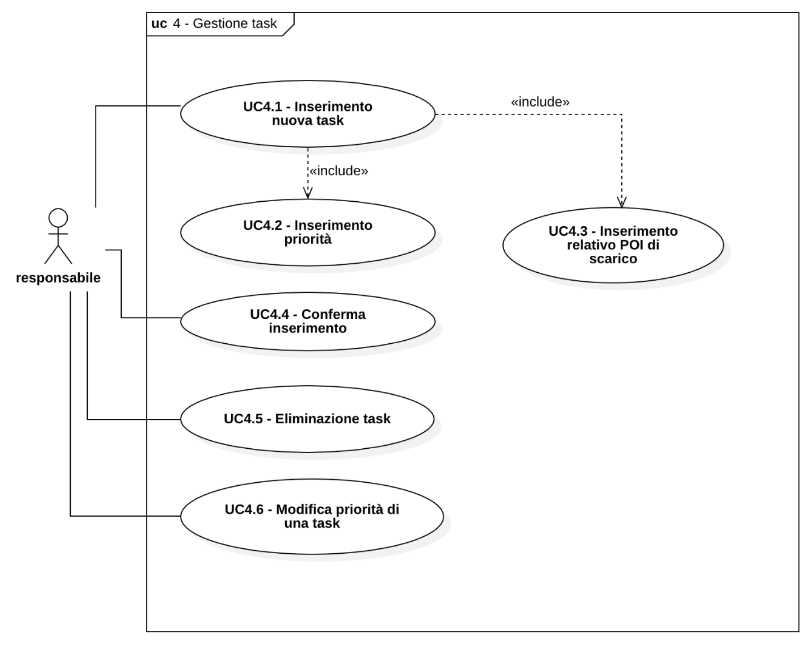
\includegraphics[scale=0.5]{res/images/esempio_use_case.png}
                    \caption{Esempio di caso d'uso}
                \end{figure}

            \ssubparagraph{Classificazione dei requisiti}
                Per favorire l'organizzazione ed il tracciamento dei \glspl{requisito}\textsubscript{G}, questi saranno classificati secondo la convenzione che segue:
                $$\text{R[tipo]-[numero progressivo]-[importanza]}$$
                dove tipo è uno tra:
                \begin{itemize}
                    \item \textbf{V}$\rightarrow$ vincolo;
                    \item \textbf{F}$\rightarrow$ funzionale;
                    \item \textbf{Q}$\rightarrow$ qualità;
                    \item \textbf{P}$\rightarrow$ prestazionale;
                \end{itemize}
                mentre importanza può essere:
                \begin{itemize}
                    \item \textbf{O}$\rightarrow$ obbligatorio, irrinunciabile per qualcuno degli \gls{stakeholder}\textsubscript{G};
                    \item \textbf{D}$\rightarrow$ desiderabile, non strettamente necessario, ma se ne riconosce il valore aggiunto;
                    \item \textbf{F}$\rightarrow$ facoltativo, relativamente utile oppure contrattabile in futuro.
                \end{itemize}
                Il numero progressivo parte da 1 ed i sotto \glspl{requisito}\textsubscript{G} si indicano in maniera analogo ai sotto \glspl{usecase}\textsubscript{G}.

        \paragraph{Progettazione}
            \ssubparagraph{Descrizione}
                I progettisti hanno il compito di tradurre il problema in una possibile soluzione, descritta come architettura, da dividere in parti che possono essere trattate individualmente. Sarà necessario:
                \begin{itemize}
                    \item svolgere le \gls{attivita}\textsubscript{G} coerentemente con quanto individuato nell'analisi dei \glspl{requisito}\textsubscript{G};
                    \item adottare \gls{designpattern}\textsubscript{G} opportuni quando si individuano strutture che ne possono trarre beneficio;
                    \item seguire i principi SOLID\footnote{\url{https://www.math.unipd.it/~rcardin/swea/2021/SOLID\%20Principles\%20of\%20Object-Oriented\%20Design_4x4.pdf}};
                    \item utilizzare sempre una nomenclatura significativa, parlante e consistente.
                \end{itemize}
            \ssubparagraph{Obiettivi di qualità}
                Affinché un'architettura si possa definire buona, deve perseguire i seguenti obiettivi di qualità: \footnote{\url{https://www.math.unipd.it/~tullio/IS-1/2020/Dispense/L09.pdf} \S\ 17..27}
                \begin{itemize}
                    \item \textbf{sufficienza: }soddisfa tutti i \glspl{requisito}\textsubscript{G};
                    \item \textbf{comprensibilità: }per tutti gli \gls{stakeholder}\textsubscript{G};
                    \item \textbf{modularità: }suddivisa in parti chiare e ben distinte;
                    \item \textbf{robustezza: }capace di sopportare ingressi diversi da utenti ed ambienti differenti;
                    \item \textbf{flessibilità: }permette modifiche a costo contenuto al variare dei \glspl{requisito}\textsubscript{G};
                    \item \textbf{riusabilità: }le sue parti possono essere impiegate in altre applicazioni;
                    \item \textbf{efficienza: }nel tempo (CPU), nello spazio (RAM), nelle comunicazioni (rete);
                    \item \textbf{affidabilità: }svolge bene il suo compito quando utilizzata con un'alta probabilità;
                    \item \textbf{disponibilità: }la sua manutenzione la rende indisponibile per un tempo ridotto;
                    \item \textbf{ \gls{safety}\textsubscript{G} };
                    \item \textbf{ \gls{security}\textsubscript{G} };
                    \item \textbf{semplicità: }ogni parte contiene solo il necessario e niente di superfluo;
                    \item \textbf{incapsulazione: }l'interno delle componenti non è visibile all'esterno;
                    \item \textbf{coesione: }le parti che stanno insieme hanno gli stessi obiettivi;
                    \item \textbf{basso accoppiamento: }parti distinte hanno una dipendenza il più possibile ridotta.
                \end{itemize}
            \ssubparagraph{Attività}
                La progettazione porterà in seguito alla produzione di una \gls{techbase}\textsubscript{G} e di una \gls{prodbase}\textsubscript{G}. A supporto di queste, ci saranno diversi diagrammi, sempre secondo lo standard \acrshort{uml}\textsubscript{A} 2.0:
                \begin{itemize}
                    \item \textbf{delle classi\footnote{\url{https://www.math.unipd.it/~rcardin/swea/2021/Diagrammi\%20delle\%20Classi_4x4.pdf}}: }per rappresentare oggetti e relazioni tra questi in un sistema;
                    \item \textbf{dei package\footnote{\url{https://www.math.unipd.it/~rcardin/swea/2021/Diagrammi\%20dei\%20Package_4x4.pdf}}: }per rappresentare dipendenze tra classi e package ad un livello di astrazione più alto rispetto a quello dei diagrammi delle classi;
                        \item \textbf{delle attività\footnote{\url{https://www.math.unipd.it/~rcardin/swea/2021/Diagrammi\%20di\%20Attivit\%c3\%a0_4x4.pdf}}: }per descrivere processi o algoritmi;
                    \item \textbf{di sequenza\footnote{\url{https://www.math.unipd.it/~rcardin/swea/2021/Diagrammi\%20di\%20Sequenza_4x4.pdf}}: }la collaborazione di un gruppo di oggetti che devono implementare collettivamente un comportamento.
                \end{itemize}
                Si dovranno indicare le tecnologie che si andranno ad utilizzare, descrivendo il loro impiego e le motivazioni che hanno portato alla loro scelta.
        \pparagraph{Codifica}
            Qui verranno definite le norme che i programmatori dovranno seguire, di modo da:
             \begin{itemize}
                 \item perseguire: leggibilità, uniformità e consistenza;
                 \item agevolare: verifica, validazione e manutenzione.
             \end{itemize}
    %\subsubsection{Strumenti}

    \pagebreak

    \section{Processi di Supporto}
\label{supporto}
\subsection{Documentazione}
    \subsubsection{Scopo}
        Lo scopo del processo di documentazione è regolamentare la creazione e la gestione dei documenti e fissare le modalità di stesura ed approvazione degli stessi.
    \subsubsection{Aspettative}
        Avere un approccio condiviso ed uniforme per la stesura e l'aggiornamento dei documenti all'interno del gruppo di lavoro è fondamentale per rendere la documentazione uno strumento costruttivo e di supporto, e non un mera formalità aggiuntiva.
        Inoltre fornire un aspetto uniforme attraverso tutti i documenti facilita qualunque lettore.
    \subsubsection{Descrizione}
        Il gruppo \group si doterà di due categorie di documentazione:
        \begin{itemize}
            \item \textbf{formale: }documenti interni o esterni che rispetteranno strettamente i vincoli descritti in seguito e che saranno interamente pubblici, realizzati in \LaTeX{} aderendo ad un template condiviso;
            \item \textbf{informale: }documenti interni che potranno svolgere diverse funzioni, tra cui:
            \begin{itemize}
                \item  raccolta appunti e ordini del giorno per riunioni;
                \item  raccolta argomenti delle discussioni delle riunioni, per tracciare l'evoluzione delle stesse e favorire la stesura dei verbali in seguito;
                \item  creazione di \gls{wiki}\textsubscript{G} per condivisione di materiale utile riguardo l'uso di tecnologie o strumenti a supporto di qualsiasi attività.
            \end{itemize}
            Questi documenti saranno realizzati sfruttando \href{https://www.atlassian.com/software/confluence}{Confluence} per garantire semplicità, accentramento e condivisione real-time.

        \end{itemize}
    \subsubsection{Ciclo di vita dei documenti}
    \label{ciclovitadoc}
        Ogni documento formale si redige ed incrementa tramite queste attività:
        \begin{itemize}
            \item \textbf{stesura: }la scrittura del documento in sé, riguarda sia la creazione di nuove parti che l'aggiornamento di queste. Uno o più redattori si occupano di ciò;
            \item \textbf{verifica: }eseguita da uno o più verificatori, necessariamente diversi dai redattori, consiste nel controllo della correttezza sintattica, semantica, grammaticale ed ortografica e della conformità del documento rispetto alle suo scopo. Nel caso in cui si rendano necessarie modifiche sostanziali, i verificatori notificheranno il responsabile che provvederà a riportare il documento in stesura e solleciterà i redattori affinché apportino le correzioni richieste;
            \item \textbf{approvazione: }quando i verificatori riporteranno la completa correttezza ed aderenza ai requisiti del documento, il responsabile provvederà all'approvazione finale ed al rilascio di una nuova versione dello stesso.
        \end{itemize}
        Adottando un approccio incrementale, queste attività possono ripetersi.
    \subsubsection{Struttura dei documenti formali}
        \pparagraph{Organizzazione in file e cartelle}
            Ogni documento, ha una sua cartella dedicata, all'interno della quale ci devono essere:
            \begin{itemize}
                \item \textbf{file principale del documento: }(nome\_documento.tex) che contiene l'impostazione della struttura, le dichiarazioni per importare i package \LaTeX{} aggiuntivi e le dichiarazioni di inclusione delle sezioni e del glossario;
                \item \textbf{cartella config: }contenente file di configurazione relativi al documento, che consentono l'impostazione del frontespizio e del registro delle modifiche;
                \item \textbf{cartella res: }per contenere le risorse del documento, a sua volta questa contiene:
                    \begin{itemize}
                        \item \textbf{cartella images: }per le eventuali immagini;
                        \item \textbf{cartella sections: }che contiene tutte le sezioni, ognuna in un file diverso, i quali seguono la convenzione di nomenclatura preceduta da un identificativo numerico progressivo ad indicare la posizione della stessa nel documento (e.g.: 01\_introduzione.tex, 02\_sezione1.tex)
                        %todo add link convenzione nomi
                    \end{itemize}
                \item \textbf{file glossario.txt: }dove definire tutti gli acronimi e le voci di glossario, che verranno poi processate \hyperref[glossario]{dall'automazione}.
            \end{itemize}
        \pparagraph{Frontespizio}
            Fornisce dele informazioni generali e di introduzione al documento, ed è così composto:
            \begin{itemize}
                \item logo esteso del gruppo;
                \item nome del documento;
                \item nome del gruppo e del progetto relativo al capitolato scelto;
                \item indirizzo email di riferimento del gruppo;
                \item versione del documento, secondo la \hyperref[versions]{convenzione};
                \item stato, in accordo con quanto descritto nel \hyperref[ciclovitadoc]{ciclo di vita dei documenti};
                \item elenco dei redattori;
                \item elenco dei verificatori;
                \item nome del responsabile che ha effettuato l'ultima approvazione
                \item destinatari del documento
                \item breve descrizione
            \end{itemize}
        \pparagraph{Registro delle modifiche}
            Raccoglie in forma tabellare tutte le modifiche e conseguentemente la storia del documento, così strutturate:
            \begin{itemize}
                \item versione del documento relativa alla modifica
                \item breve descrizione delle attività svolte
                \item data della modifica, secondo lo standard \href{https://www.iso.org/iso-8601-date-and-time-format.html}{ISO 8601}
                \item cognome e nome di chi ha apportato la modifica
                \item ruolo del modificatore rispetto al ciclo di vita del documento, può quindi essere: redattore, verificatore, responsabile.
            \end{itemize}
        \pparagraph{Indice}
            Riassume i contenuti del documento raccolti per sezioni ed intestazioni, indicando la pagina di inizio e collegando alla stessa
        \pparagraph{Elenchi delle figure e tabelle}
            Nel caso in cui un documento presenti una o più figure o tabelle, queste sezioni le indicheranno raccogliendole rispettivamente ed indicando la pagina di apparizione.
        \pparagraph{Sezione di introduzione}
            La prima sezione di contenuto di ogni documento formale è l'introduzione che si articola in:
            \begin{itemize}
                \item una sezione che descrive lo scopo del documento;
                \item due sezioni condivise fra tutti i documenti, non verbali, che illustrano rispettivamente scopo del prodotto del capitolato scelto e funzionamento di acronimi, voci di glossario e riferimenti ad altri documenti;
                \item una sezione che contiene tutti i riferimenti, di natura normativa o informativa.
            \end{itemize}
        \pparagraph{Ulteriori sezioni, appendici e glossari}
            Come indicato precedentemente ogni sezione di primo livello deve avere un suo file dedicato e si svilupperà in seguito all'introduzione. Al termine di tutte le sezioni vi può essere un'appendice mentre le ultime pagine elencano la lista degli acronimi e i termini di glossario utilizzati nel documento, con riferimenti alle pagine dove questi appaiono.

        \subsubsection{Verbali}
            I verbali possono essere interni, se relativi ad una riunione dei soli membri del gruppo, o esterni, se relativi ad un qualche tipo di incontro con persone esterne al gruppo. Come gli altri documenti formali, hanno un frontespizio ed un registro delle modifiche, poi si articolano in questo modo:
            \begin{itemize}
                \item informazioni generali
                    \subitem -- dettagli sull'incontro
                        \subsubitem -- luogo, data\footnote{Standard ISO 8601}, orari di inizio e fine e partecipanti
                    \subitem -- ordine del giorno;
                \item verbale della riunione
                    \subitem -- contiene tutte le sottosezioni necessarie a descrivere lo svolgimento dell'incontro;
                \item conclusioni
                    \subitem -- nel caso di verbale interno, una tabella di tracciamento delle decisioni;
                    \subitem -- nel caso di verbale esterno, un paragrafo riassuntivo.
            \end{itemize}
            Ogni verbale avrà come nome "verbale\_[tipo]\_[num]" dove tipo può essere interno o esterno, e num e il progressivo rispetto al tipo.
            \pparagraph{Tracciamento delle decisioni nei verbali interni}
                Ogni riga della tabella di tracciamento delle decisioni si compone di:
                \begin{itemize}
                    \item \textbf{codice: }indentificativo univoco della decisione, così formato: VI\_numRiunione.numDecisione (e.g.: VI\_2.3 indica la terza decisione presa durante la riunione interna 2);
                    \item \textbf{decisione: }breve riassunto che indichi in maniera chiara la decisione presa.
                \end{itemize}
        \subsubsection{Glossario e acronimi}
            Ogni documento ha una sua sezione dedicata al glossario e agli acronimi a fine documento, dove sono indicate anche le pagine di apparizione delle rispettive voci.
            \pparagraph{Definzione ed utilizzo delle voci}
                Gli acronimi ed i termini di glossario vanno definiti nel glossario.txt, istruzioni precise su come utilizzare correttamente questo documento si trovano nella \textsc{wiki how-to glossario}. Una volta che una voce è stata aggiunta, la si può usare liberamente in qualsiasi sezione tramite il suo nome, singolare o plurale nel caso di termine nel glossario, o abbreviazione nel caso di acronimo

            \pparagraph{Funzionamento}
                Ad ogni azione di \gls{gitpush}\textsubscript{G} su un branch feature, un'automazione \href{https://docs.github.com/en/free-pro-team@latest/actions}{github action} si occupa di eseguire uno script \gls{bash}\textsubscript{G}, glossary\_builder.sh il quale:
                \begin{itemize}
                    \item controlla tutti i documenti che hanno un glossario.txt;
                    \item ne genera un glossario.tex;
                    \item sostituisce tutte le occorrenze delle voci di glossario e acronimi in ogni sezione con i rispettivi comandi \LaTeX{}
                    \item se ci sono stati cambiamenti, ricompila il glossario e ricompila il documento per ottenere un pdf aggiornato;
                    \item se ci sono stati dei documenti aggiornati, effettua \gls{gitcommit}\textsubscript{G} e \gls{gitpush}\textsubscript{G}.
                \end{itemize}
                Questo permette di avere sempre i file pdf dei documenti aggiornati e con le voci di glossario correttamente compilate e collegate, in maniera automatica e rapida. Si consiglia quindi ai membri di effettuare sempre una \gls{gitpull}\textsubscript{G} prima di apportare nuove modifiche ai documenti se si ha precedentemente eseguito una \gls{gitpush}\textsubscript{G}, così da avere il documento aggioranto ed evitare problemi di conflitti e nel \acrshort{vcs}\textsubscript{A}.
        \subsubsection{Norme tipografiche}
            \pparagraph{Nomi di file e cartelle}
                Ogni file e cartella dovrà avere un nome:
                \begin{itemize}
                    \item che sia il più possibile conciso ed esplicativo;
                    \item composto di sole lettere minuscole, numeri, \_ e '-', ad eccetto del '.' per separare nome da estensione
                    \item che abbia alla fine un'estensione coerente col suo tipo
                    \item non contenere spazi o caratteri diversi da quelli indicati sopra, parole diverse si separano con '\_'
                \end{itemize}
            \pparagraph{Stile del testo}
                Ai seguenti stili si attribuisce una specifica funzione semantica:
                \begin{itemize}
                    \item \textbf{corsivo: }per denotare termini tecnici appartenenti ad una particolare tecnologia che si sta trattando;
                    \item \textbf{grassetto: }per evidenziare termini rilevanti o dei quali viene dato un significato esteso immediatamente in seguito, come questi in un elenco puntato;
                    \item \textbf{maiuscoletto: }per indicare altri documenti (e.g.: \textsc{Piano di Progetto});
                    \item \textbf{pedice: } G e A, per indicare rispettivamente una voce di glossario o un acronimo.
                \end{itemize}
            \pparagraph{Elenchi}
                Ogni elemento deve terminare con un punto e virgola, eccetto quella finale che va seguito da un punto, quindi ogni prima parola deve avere iniziale minuscola a meno che non indichi qualcosa per la quale la capitalizzazione è importante. Gli elenchi puntati non numerati avranno come simbolo di primo livello un puntino pieno, come secondo un trattino, come terzo un asterisco. Gli elenchi numerati come primo livello numeri, come secondo lettere minuscole, come terzo numeri romani rappresentati con lettere minuscole
                \begin{multicols}{2}
                    \begin{itemize}
                        \item elenco puntato non numerato
                        \item secondo elemento
                        \begin{itemize}
                            \item secondo livello
                            \begin{itemize}
                                \item terzo livello
                            \end{itemize}
                        \end{itemize}
                    \end{itemize}
                    \begin{enumerate}
                        \item elenco puntato numerato
                        \item secondo elemento
                        \begin{enumerate}
                            \item secondo livello
                            \begin{enumerate}
                                \item terzo livello
                            \end{enumerate}
                        \end{enumerate}
                    \end{enumerate}
                \end{multicols}
                \centerline{(Esempi elenchi puntati numerati e non corretti)}
            \pparagraph{Data e ora}
                In ogni documento si adotta lo \href{https://www.iso.org/iso-8601-date-and-time-format.html}{Standard ISO 8601} , quindi aaaa-mm-gg (e.g.: 5 Gennaio 2021 = 2021-01-05) e hh:mm. Se si scrive il mese in caratteri questo con l'iniziale maiuscola e vale lo stesso per i giorni della settimana.
            \pparagraph{Codici di versioni}
            \label{versions}
                % non trovato standard ufficiale, solo https://semver.org/ ma sempre essere più per il codice e basta e comunque introduce molte complicazioni
                Si adotta la convenzione $x.y.z$ dove x, y e z sono numeri progressivi che partono da 0, x non si azzera mai, y si azzera ad ogni incremento di x e z si azzera ad ogni incremento di y o x. Gli incrementi avvengono:
                \begin{itemize}
                    \item \textbf{per x: }quando avviene un accertamento da parte del responsabile di modifiche sostanziali
                    \item \textbf{per y: }quando viene apportato un insieme discreto di modifiche;
                    \item \textbf{per z: }per ogni modifica o verifica minore.
                \end{itemize}

        \subsubsection{Strumenti}
            Come già citato, per la scrittura dei documenti formali si usa \LaTeX\footnote{https://www.latex-project.org/} e come editor non c'è una preferenza assoluta, ma si consigliano \href{http://www.texstudio.org/}{TexStudio} o \href{https://www.xm1math.net/texmaker/}{TexMaker}. Per quanto riguarda i documenti informali invece, \href{https://www.atlassian.com/software/confluence}{Confluence} può essere usato in qualunque browser.


\subsection{Gestione della configurazione}
    \subsubsection{Scopo}
        Lo scopo del processo di gestione della configurazione è quello di applicare procedure amministrative e tecniche al fine di controllare e registrare modifche e rilasci ed assicurare la correttezza, consistenza, completezza ed archiviazione di ogni elemento.
    \subsubsection{Aspettative}
        Avere uno spazio di lavoro versionato, condivisp ed altamente orientato alla collaborazione è fondamentale in gruppo di lavoro con molteplici componenti. La storicizzazione, tracciabilità e reversibilità di ogni cambiamento permettono di concentrarsi sulla produzione di nuovo valore invece che sulle problematiche di versionamento, conflitti e condivisione.
    \subsubsection{Descrizione}
        Il gruppo \group ha un organizzazione su github\footnote{\group su Github: \url{https://github.com/Three-Way-Milkshake}} all'interno della quale gestisce tutte le \acrshort{repo}\textsubscript{A} di cui necessita.
    \subsubsection{Workflow di versionamento}
        Il gruppo adotta il workflow \href{https://www.atlassian.com/git/tutorials/comparing-workflows/gitflow-workflow}{gitflow} all'interno di ciascuno \acrshort{repo}\textsubscript{A}. Per semplificare le operazioni si può usare il pacchetto di estensioni \href{http://danielkummer.github.io/git-flow-cheatsheet/}{git-flow}. Maggiori informazioni ed istruzioni per l'uso di \gls{git}\textsubscript{G} e GitHub si trovano nella \gls{wiki}\textsubscript{G} \textsc{GIT, Github \& Jira}
        \pparagraph{Pull requests}
            Per l'implementazione delle feature dai branch di lavoro, bisogna aprire una \gls{gitpull}\textsubscript{G} request su develop. A questo punto il responsabile o l'amministratore provvederanno a fare i controlli necessari ed effettueranno il merge\footnote{Il merge in \gls{git}\textsubscript{G}: \url{https://www.atlassian.com/git/tutorials/using-branches/git-merge}} tramite \textit{squash}.

    \subsubsection{Integrazione con Jira}
    \label{jiraintegration}
        GitHub è stato configurato in maniera che ad ogni commit si scatenino delle azioni che coinvolgono Jira. Usando una specifica sintassi\footnote{\url{https://support.atlassian.com/bitbucket-cloud/docs/use-smart-commits/}} \footnote{wiki \textsc{GIT, Github \& Jira}} è possibile collegare ogni commit con una task o sottotask di Jira, aggiungendo direttamente su questa commenti, tracciamento del tempo di lavoro ed apportando modifiche allo stato di progresso.

    \subsubsection{Strumenti}
        Come già detto, le \acrshort{repo}\textsubscript{A} sono tenute su GitHub, per quanto riguarda la gestione locale, ogni membro è libero di adottare lo strumento che preferisce.

\subsection{Accertamento della qualità} %todo
    \subsubsection{Scopo}
        Lo scopo del processo di ...
    \subsubsection{Aspettative}
        ...
    \subsubsection{Descrizione}
        ...
    \subsubsection{altre sottosezioni}
        ...

\subsection{Verifica} %todo
\label{verifica}
    \subsubsection{Scopo}
        Lo scopo del processo di ...
    \subsubsection{Aspettative}
        ...
    \subsubsection{Descrizione}
        ...
    \subsubsection{altre sottosezioni}
        ...
    \subsubsection{Strumenti}
        ...


\subsection{Validazione} %todo
    \subsubsection{Scopo}
        Lo scopo del processo di ...
    \subsubsection{Aspettative}
        ...
    \subsubsection{Descrizione}
        ...
    \subsubsection{altre sottosezioni}
        ...
    \subsubsection{Strumenti}
        ...

\subsection{Risoluzione dei problemi}
\label
    \subsubsection{Scopo}
        Questo processo ha lo scopo di definire un insieme di procedure atte alla risoluzione dei problemi.
    \subsubsection{Aspettative}
        Identificazione, segnalazione e risoluzione dei problemi devono avvenire in maniera standardizzata all'interno del gruppo così che tutto il processo possa essere svolto nei tempi più brevi possibili.
    \subsubsection{Descrizione}
        Quando un verificatore riscontra dei problemi, tramite il meccanismo degli \hyperref[jiraintegration]{\textit{smart commits}}, riporta la task o sottotask relativa al problema individuato nello stato \textit{in progress} ed aggiunge un commento che indica i problemi riscontrati. Nel caso sia necessario aggiungere più informazioni, il verificatore si può recare nella board ed aggiungere ulteriori commenti. Il verificatore viene quindi sollevato automaticamente dal compito, il responsabile controlla il problema segnalato, se necessario imposta una priorità diversa da \textit{medium}, aggiunge eventuali commenti o descrizioni e riassegna la task ad un altro membro. Il responsabile può sfruttare le sezioni \textit{history} e \textit{comments} di ogni task per controllare chi ha lavorato in passato a quel compito di modo da facilitare la scelta di assegnazione.
    \pagebreak

    \section{Processi Organizzativi}
\label{organizzativi}

\subsection{Gestione dei processi}
    \subsubsection{Scopo}
    Qui lo scopo è la gestione delle attività\textsubscript{G} e dei compiti per ogni altro processo.
    \subsubsection{Aspettative}
    L'organizzazione e la gestione dei compiti all'interno del gruppo di lavoro deve avvenire in modo sistematico\textsubscript{G}, disciplinato\textsubscript{G} e quantificabile\textsubscript{G} così da favorire uno svolgimento dei lavori ordinato, che rispetti i tempi e che non sia vulnerabile a variazioni e problemi che si possono certamente riscontrare.
    \subsubsection{Descrizione}
    Il responsabile e l'amministratore si sono occupati della creazione e della configurazione di tutti gli ambienti necessari:
    \begin{itemize}
        \item account gmail;
        \item organizzazione GitHub;
        \item calendario condiviso su Google Calendar;
        \item workspace \href{https://slack.com/intl/en-it/about}{Slack};
        \item workspace Confluence con spazio dedicato ai verbali e spazio dedicato alle wiki\textsubscript{G};
        \item progetto\textsubscript{G} Jira con board condivisa per l'organizzazione, gestione e tracciamento dei compiti;
        \item organizzazione del cruscotto\textsubscript{G} contenete varie informazioni sull'andamento del progetto\textsubscript{G}, presente su Google Sheet;
        \item organizzazione di un sito per la visualizzazione del cruscotto\textsubscript{G}, tramite Google Sites;
        \item organizzazione di Google Drive.
    \end{itemize}
        \pparagraph{Jira}
        Il gruppo adotta \href{https://www.atlassian.com/software/jira}{Jira} per la gestione dei compiti, così da avere:
        \begin{itemize}
            \item cruscotto\textsubscript{G} di lavoro che mostri lo stato di ogni compito:
                \subitem -- ogni task\textsubscript{G} ha diversi campi oltre al nome (descrizione, data di scadenza, assegnatari, eventuali sottotask), comprende una sezione \textit{history} che raccoglie tutte le modifiche avvenute sulla stessa, una sezione \textit{comments} che raccoglie commenti apportati manualmente o automaticamente importati dagli \textit{smart commits} ed una sezione per il tracciamento del tempo, nel quale si può impostare un tempo stimato e tracciare quello effettivo mano a mano che si prosegue;
            \item integrazione con Confluence, essendo entrambi prodotti di \href{https://www.atlassian.com/}{Atlassian};
            \item automazioni per azioni con gli \textit{smart commits};
            \item automazioni di notifiche su Slack.
        \end{itemize}
        Come spiegato nella sezione \hyperref[jiraintegration]{Integrazione con Jira}, è stato configurato un processo automatico di collegamento fra commit\textsubscript{G} su GitHub e task\textsubscript{G} in Jira. Inoltre ad ogni azione, manuale o automatica, su Jira, viene generata una notifica nel canale dedicato di Slack.
        \pparagraph{Workflow dei compiti}
        \begin{figure}[H]
            \centering
            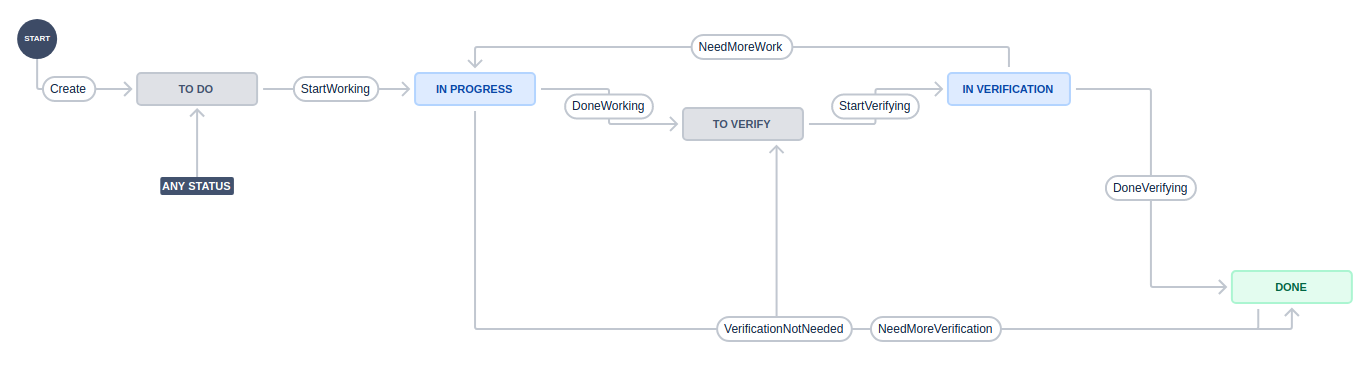
\includegraphics[scale=0.32]{res/images/jira_workflow.png}
            \caption{Diagramma degli stati e delle transizioni del workflow}
        \end{figure}
            Come si può vedere dall'immagine, il workflow di task\textsubscript{G} e sottotask è stato configurato di modo che ci siano delle precise transizioni da uno stato all'altro e che solo quelle siano permesse. I nomi delle transizioni sulle frecce corrispondono ai comandi da usare nella sintassi degli smart commit\textsubscript{G}. Maggiori dettagli si trovano nella wiki\textsubscript{G} \textsc{Git, Github \& Jira}.
        \pparagraph{Google Sheet}
        Si fa uso del foglio elettronico di Google Sheet per tenere traccia di tutte le informazioni relative alle metriche usate nel \textsc{Piano di Qualifica}. Contiene dati essenziali al controllo dello svolgimento del progetto\textsubscript{G}, come il tempo per ogni lavoro individuale svolto dal singolo soggetto o il tempo effettivo e preventivato di una specifica riunione. Parte di questo foglio è stato bloccato in maniera tale da favorire l'inserimento dei soli dati da parte dei componenti del gruppo.
        
        \pparagraph{Google Sites}
        Collegato direttamente con i grafici del cruscotto\textsubscript{G} presente in Google Sheet, il sito interattivo creato tramite Google Sites permette di avere una rapida visualizzazione dell'avanzamento del progetto\textsubscript{G}. Questo sito, diviso in periodi, propone delle "fotografie" ritraenti degli specifici grafici utili a verificare velocemente metriche essenziali del \textsc{Piano di Qualifica} e la loro variazione tra periodi diversi.
        
        \pparagraph{Google Drive}
        Viene utilizzato uno spazio Google Drive per contenere tutti i file utili al gruppo, come presentazioni, materiale utile alla comprensione delle tecnologie da utilizzare, un foglio elettronico contenente le varie metriche per \textsc{Piano di Qualifica} e diagrammi \href{https://drawio-app.com/}{Draw.io}
        
        \pparagraph{Workflow per l'inizio di una nuova task}
        \begin{enumerate}
        	\item Si prende il codice della task\textsubscript{G} da Jira: PCS-\#\#\# e si va sull’Excel \textbf{Sincronizzazione Dati} nella riga corrispondente \textbf{TEMPO (minuti) PREVENTIVATO} → tempo durata preventivato (relativo al lavoro);
        	\item in \textbf{ATA \#StartWorking → \#DoneWorking: }
        	\begin{itemize}
        		\item Settare date: \textbf{AVVIO} e \textbf{SCADENZA PREFISSATA};
        		\item Ogni qualvolta si committa con 'git commit\textsubscript{G} -m “PCS-\#\#\# \#comment <commento> \#time <tempo>” ' (quindi usando tracciamento temporale di Jira) e si incrementa sull’excel.
        	\end{itemize}
        	\item Al termine del lavoro della task\textsubscript{G} si dovrà andare ad inserire la data di fine effettiva della colonna \textbf{DATA \#StartWorking → \#DoneWorking FINE EFFETTIVA};
        	\item Aggiungere il \textbf{TEMPO (minuti) EFFETTIVO} con relativo \textbf{Ruolo};
        	\item quando finito controllare \url{https://threewaymilkshake.atlassian.net/wiki/spaces/VER/pages/138412040/Sequenza+Stesura+e+Verifica+verbali} e assegnare la verifica a chi tocca, secondo l’ordine.
        \end{enumerate}
    	
    	\pparagraph{Workflow per la verifica di una task}
    	\begin{enumerate}
    		\item Si prende il codice della task\textsubscript{G} da Jira: PCS-\#\#\# e si va sull’Excel \textbf{Sincronizzazione Dati} nella riga corrispondente \textbf{TEMPO (minuti) PREVENTIVATO} → tempo durata preventivato (relativo alla verifica);
    		\item settare \textbf{SCADENZA PREFISSATA} in \textbf{DATA \#StartVerifying → \#DoneVerifying};
    		\item Al termine della verifica si dovrà andare ad inserire la data di fine effettiva della colonna \textbf{DATA \#StartVerifying → \#DoneVerifying AVVIO (=EFFETTIVA FINE DI \#TOVERIFY) FINE EFFETTIVA}.
    	\end{enumerate}
    
    	\pparagraph{Workflow per le riunioni}
    	Chi dovrà redigere il verbale dovrà::
    	\begin{enumerate}
    		\item In \textbf{Durata Riunioni - Dati} inserire la \textbf{Data, Prevista ed Effettiva}  sotto \textbf{Durata riunioni interne / esterne};
    		\item Creare branch feature/VT-n con T → {I, E}, n → numero
    		\item Quando finito, oltre a settare tempi come per task\textsubscript{G} normali, controllare file in \url{https://threewaymilkshake.atlassian.net/wiki/spaces/VER/pages/138412040/Sequenza+Stesura+e+Verifica+verb} e:
    		\begin{itemize}
    			\item Spuntare la propria box;
    			\item Una volta che la task\textsubscript{G} è in toVerify con l’assignee cancellato (si cancella da solo tramite automazione) assegnare a chi tocca la verifica.
    		\end{itemize}
    		\item Spostare note su Confluence → Trascritti.
    	\end{enumerate}

\subsection{I ruoli di progetto}
    La suddivisione in ruoli è necessaria per favorire la parallelizzazione e distribuzione del lavoro e delle responsabilità.
    \subsubsection{Analista}
    Hai il compito specifico di comprendere il problema. Ha un ruolo attivo fin quando la comprensione non è adeguata. Adottando un modello incrementale\textsubscript{G}, rimane più a lungo ed evolve. E auspicabile che ci siano più analisti per portare punti di vista diversi e sommare le conoscenze. Redige \textsc{Studio di Fattibilità} ed \textsc{Analisi dei Requisiti}.
    \subsubsection{Progettista}
    Traduce il problema in una possibile soluzione, descritta come architettura, divisa in parti per agevolare lo sviluppo individuale di queste. Dati i vincoli ha il compito di trovare una buona soluzione. Redige le specifiche tecniche e le definizioni del prodotto.
    \subsubsection{Verificatore}
    Agisce su ogni attività\textsubscript{G} ed attua una verifica oggettiva, segnalando eventuali problemi secondo il \hyperref[label]{text}{processo rispettivo}.
    \subsubsection{Programmatore}
    Implementa in codice ciò che i progettisti hanno definito come design. Un'adeguata divisione dei compiti tra diversi programmatori consente un alto parallelismo, ideale per avanzare rapidamente. Deve svolgere compiti piccoli, che siano facilmente verificabili.
    \subsubsection{Responsabile}
    Gestisce il controllo sul progetto\textsubscript{G} e tramite un cruscotto\textsubscript{G} di controllo aggiorna, revisiona ed adatta lo svolgimento dei lavori. Elabora piani e scadenze, assegna compiti, approva documenti, gestisce i problemi, redige l'\textsc{Organigramma} ed il \textsc{Piano di Progetto} ed approva l'offerta prima di sottoporla al committente.
    \subsubsection{Amministratore}
    Ha in carico la definizione, modifica ed agevolazione del way of working. È un percorso in logica JiT\textsubscript{A} procede per incrementi. È responsabile dell'efficacia e dell'efficienza nell'ambiente di lavoro, gestisce la documentazione, organizza il glossario, collabora alla redazione del \textsc{Piano di Progetto} e redige le \textsc{Norme di Progetto}.

\subsection{Gestione delle comunicazioni}
    Di seguito si definiscono le procedure e gli strumenti adottati per standardizzare ed organizzare le comunicazioni all'interno ed all'esterno del gruppo.
    \subsubsection{Comunicazioni interne}
        Riguardano i soli componenti del gruppo \group e in base allo scopo si articolano tramite strumenti diversi.
        \pparagraph{Google meet}
            Piattaforma di videoconferenze\footnote{\url{https://meet.google.com/}} di Google che permette la condivisione di più schermi e non richiede l'installazione di programmi aggiuntivi in quanto fruibile da browser. Integrata con Google Calendar permette la creazione di meeting collegati ad eventi direttamente da quest'ultimo strumento, semplificando così il processo di creazione ed organizzazione di eventi comuni.
            Viene utilizzata per le riunioni, le quali devono essere effettuate con una frequenza non inferiore a quella settimanale. Per ogni riunione il gruppo segue l'ordine del giorno che si sarà venuto a formare nel documento Confluence dedicato allo specifico incontro, al quale tutti possono collaborare. Le discussioni e le decisioni verranno raccolte dal segretario, che cambierà ad ogni riunione, per distribuire equamente questo compito a rotazione, nello stesso documento dal quale poi produrrà il verbale seguendo le regole definite in \ref{verbali}.
        \pparagraph{Slack}
            Strumento di messaggistica fortemente orientato alla collaborazione in gruppi di lavoro \footnote{\url{https://slack.com/intl/en-it/about}}. Il gruppo \group ha un workspace dedicato nel quale sono presenti diversi canali, per suddividere ed organizzare le comunicazioni. Durante lo svolgimento del progetto\textsubscript{G} si possono creare tanti canali quanti se ne rendono necessari, il responsabile provvederà alla gestione di questi. Oltre ai canali dedicati alle attività\textsubscript{G} appena citati ci sono i seguenti:
            \begin{itemize}
                \item \textbf{generale: }per le comunicazioni che non ricadono in nessun canale specifico già esistente e per le quali non si rende ncecessaria la creazione di un nuovo canale;
                \item \textbf{capitolato-c5-portacs: }all'interno del quale l'amministratore configura le integrazioni automatizzate utili a notificare i componenti del gruppo:
                \begin{itemize}
                    \item jira, invierà una notifica ogni qualvolta che si intraprenderà un'azione, manuale o automatica (\textit{smart commits}) sul cruscotto\textsubscript{G} di progetto\textsubscript{G};
                    \item github, notificherà ogni azione intrapresa sui branch \textit{master} e \textit{develop};
                    \item google calendar, che provvederà a notificare la programmazione di eventi e ricorderà quelli imminenti allegando codice Google meet per accedere direttamente alla riunione.
                \end{itemize}
            \end{itemize}
        \pparagraph{Telegram}
            Software di messaggistica \footnote{\url{https://telegram.org/}} nel quale il gruppo \group ha un gruppo dedicato utilizzato solamente per le comunicazioni informali e non strettamente legate al progetto\textsubscript{G} di lavoro.
    \subsubsection{Comunicazioni esterne}
        Possono avvenire tra il gruppo \group ed il proponente e/o con il committente. Il gruppo si adatterà allo strumento preferito da questi in ogni momento nel quale si renda necessario il contatto. Per le comunicazioni rapide e dirette che non richiedono un incontro sincrono fra le parti, fornitore e proponente si sono accordati per l'utilizzo di uno spazio Google Chat\footnote{\url{https://workspace.google.com/products/chat/}}.

\subsection{Gestione dei Rischi}
    \subsubsection{Descrizione}
        I rischi previsti o identificati devono essere prontamente documentati nel \textsc{Piano di Progetto}. Ogni rischio dovrà essere così descritto:
        \begin{itemize}
            \item nome;
            \item \textbf{codice}: secondo la classificazione in \ref{classifrischi};
            \item \textbf{occorrenza e pericolosità: }possono assumere i valori bassa, media alta;
            \item descrizione;
            \item metodologie di rilevamento;
            \item piano di contingenza.
        \end{itemize}
    \subsubsection{Classificazione dei Rischi}
    \label{classifrischi}
        Per facilitare raccolta e riferimenti successivi, il codice identificativo di ogni rischio deve seguire la seguente convenzione:
        $$ \text{RIS\_[tipo]-[num]} $$
        dove tipo può essere:
        \begin{itemize}
            \item \textbf{T} $\rightarrow$ tecnologico;
            \item \textbf{O} $\rightarrow$ organizzativo;
            \item \textbf{I} $\rightarrow$ interpersonale;
        \end{itemize}
    mentre num è un numero progressivo che parte da 1 per ogni categoria, ed è univoco all'interno della stessa.
    \begin{figure}[H]
        \centering
        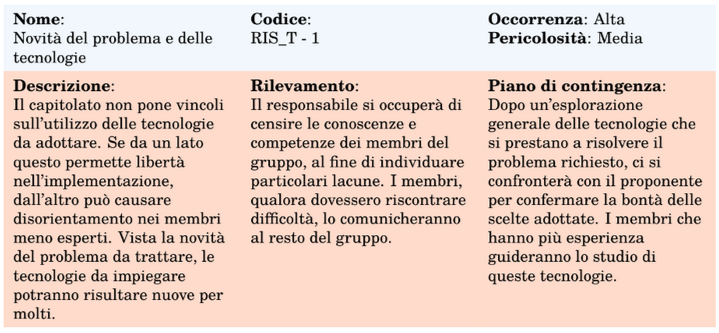
\includegraphics[scale=0.6]{res/images/esempio_rischio.png}
        \caption{Esempio corretto di raccolta rischio.}
    \end{figure}

\subsection{Formazione}
    I membri del gruppo \group sono tenuti a formarsi individualmente in quanto si ritiene che i tempi e le modalità di questo processo siano altamente individuali. Per quanto riguarda tecnologie e strumenti di interesse al gruppo, ogni membro è libero di creare una wiki\textsubscript{G} nello spazio dedicato di Confluence per raccogliere risorsa\textsubscript{G} e documentazioni utili, raccolte online o prodotte dallo stesso, così da condividere le proprie conoscenze apprese e velocizzarne l'assorbimento da parte degli altri componenti. \\
    Per i compiti attuali e per quanto discusso fino a questo momento con il proponente, si rimandano i membri del gruppo alle seguenti fonti ufficiali:
    \begin{itemize}
        \item \textbf{\LaTeX: }
            \subitem -- \url{https://www.latex-project.org/};
            \subitem -- \url{https://www.overleaf.com/learn};
        \item \textbf{Github: }\url{https://docs.github.com/en};
        \item \textbf{Confluence: }\url{https://confluence.atlassian.com/alldoc/};
        \item \textbf{Java: }\url{https://docs.oracle.com/en/java/};
        \item \textbf{Nodejs: }\url{https://nodejs.org/en/docs/}.
    \end{itemize}
	\pagebreak

    %\printglossaries
    \printglossary[type=\acronymtype,title=Lista degli Acronimi]
    \printglossary[title=Glossario dei Termini]

\end{document}
